This chapter establishes the theoretical foundation of the thesis. It first introduces flow as a psychological state and explains it through the challenge-skill model. It then summarizes physiological and behavioral correlates of flow and motivates the biometric and webcam-based signals used in this work. Building on that basis, the chapter discusses physio-adaptive systems and their practical limitations. Finally, it presents the biocybernetic control loop as the guiding architecture for closed-loop human-computer interaction.

\subsection{The Phenomenon of Flow}

The concept of \enquote{flow}, first formalized by \textcite{inbook}, describes a state of \enquote{optimal experience} in which individuals are fully absorbed in an activity. In this state, action and awareness converge, self-referential thought recedes, and the subjective perception of time is altered \autocite{nah2014flow}. According to \textcite{inbook}, this state is defined by nine distinct dimensions that characterize the depth of the experience:

\begin{enumerate}
    \item \textbf{Challenge-Skill Balance:} The task's difficulty matches the individual's high level of skill.
    \item \textbf{Action-Awareness Merging:} The individual and the activity become one; movements feel automatic.
    \item \textbf{Clear Goals:} The user understands exactly what needs to be achieved at every step.
    \item \textbf{Unambiguous Feedback:} Performance success or failure is immediately apparent, allowing for real-time adjustment.
    \item \textbf{Concentration on the Task at Hand:} A high degree of focus that excludes all irrelevant thoughts or distractions.
    \item \textbf{Sense of Control:} The user feels a sense of agency and mastery over their actions and the environment.
    \item \textbf{Loss of Self-Consciousness:} The ego recedes, and the individual stops worrying about social evaluation.
    \item \textbf{Transformation of Time:} Time is perceived differently, either appearing to speed up or slow down significantly.
    \item \textbf{Autotelic Experience:} The activity is intrinsically rewarding, meaning it is performed for its own sake rather than for an external reward.
\end{enumerate}

A central explanatory framework for achieving these dimensions is the \textbf{challenge-skill model}. The model assumes that flow emerges in a \enquote{channel} where perceived task demands are well matched to an individual's capabilities. 



While the literature describes several alternative conceptualizations—including the eight-channel model, which segments the experience into states such as arousal and apathy, and the dynamic process approach, which views flow as a longitudinal path \autocite{Moneta2012}—this thesis specifically utilizes the challenge-skill model. This selection is grounded in the model's high degree of operational utility for physio-adaptive system design. Unlike more descriptive or longitudinal models, the challenge-skill framework can be operationalized either as a tertiary structure (Boredom vs. Flow vs. Anxiety) or as a binary classification problem. In the binary case, \textit{Flow} represents the positive class, while \textit{Boredom} and \textit{Anxiety} are grouped as \textit{non-flow} states. This makes the model well suited for real-time machine learning classification. Furthermore, it aligns with the principles of Dynamic Difficulty Adjustment (DDA) in e-sports, where the primary objective is to maintain the "Flow Channel" by balancing system demands against the player's physiological responses \autocite{Moneta2012, cowley2008understanding}.


As shown in Figure~\ref{fig:challengeSkillDiagram}, an imbalance in either direction tends to move users away from flow: excessive challenge relative to skill is associated with \textbf{anxiety}, while insufficient challenge is associated with \textbf{boredom}. In e-sports contexts, this relation is often interpreted as an information-processing fit, where flow is most likely when game demands align with the player's cognitive processing capacity \autocite{cowley2008understanding}.

\begin{figure}[htbp]
    \centering
    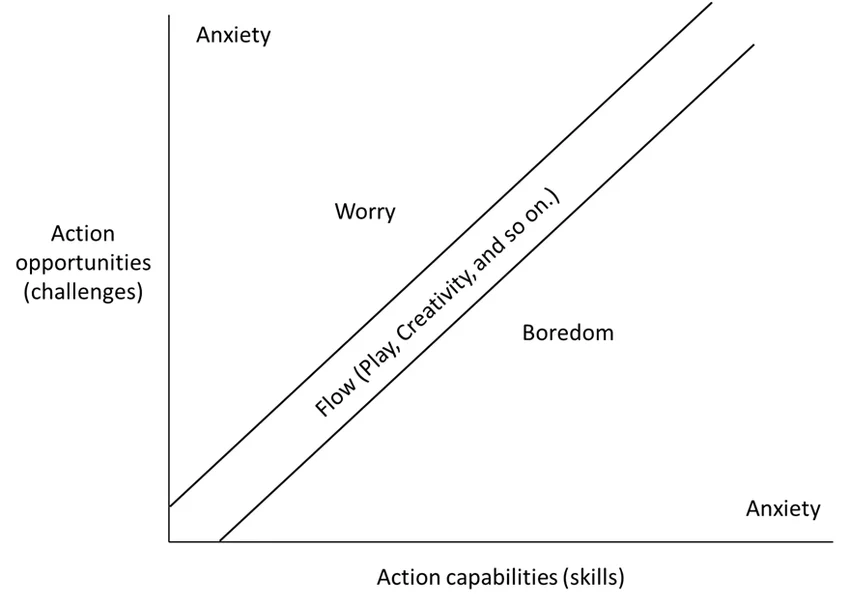
\includegraphics[width=0.72\textwidth]{flowChallenge.png}
    \caption{Challenge-skill model of flow: flow emerges when perceived challenge and perceived skill are balanced at a high level (adapted from \url{https://www.researchgate.net/figure/The-flow-channel-model-adapted-from-Csikszentmihalyi-1975_fig1_259998152}).}
    \label{fig:challengeSkillDiagram}
\end{figure}

\paragraph{Critical Analysis and Limitations of Flow Theory.}
Despite its broad adoption, flow theory has important theoretical and methodological limitations:
\begin{itemize}
    \item \textbf{Subjectivity and the measurement paradox:} Flow is commonly measured via retrospective self-reports. However, because flow involves reduced self-reflection during task execution, attempts to assess it in real time via self reports may disrupt the state itself \autocite{9296229}.
    \item \textbf{Potential maladaptive outcomes:} Although frequently framed as beneficial, prolonged flow in gaming can be linked to problematic patterns such as excessive play, social withdrawal, and neglect of basic needs (e.g., sleep and nutrition) \autocite{harris2023systematic}.
\item \textbf{Model simplification:} The linear challenge-skill representation may underdescribe competitive e-sports settings, where social pressure, team coordination, and situational volatility also shape the experience \autocite{poulus2021determinants}.\end{itemize}

\subsection{Physiological Correlates of Flow}
To complement subjective self-reports, this thesis utilizes physiological measures as objective indicators of the user's state. Other biological markers, such as cortisol, were explicitly excluded from the real-time runtime loop of the proposed prototype. While early neurophysiological studies suggested an inverted U-shaped pattern between cortisol release and flow components, its coarse temporal resolution makes it structurally unsuited for millisecond-level, closed-loop physio-adaptive interventions, which require immediate data streams.

The primary neurophysiological signals considered during model development and context mapping are:

\begin{enumerate}
    \item \textbf{Electrocardiography (ECG):} ECG records the raw electrical activity of the heart, from which \textbf{Heart Rate Variability (HRV)} is derived. While standard stress states are characterized by a purely sympathetic "fight-or-flight" response, recent literature indicates that the flow experience is uniquely characterized by a complex \textbf{dual-branch co-activation} pattern of both the sympathetic and parasympathetic nervous systems \autocite{uechtritz2026neurophysiological}. This co-activation functions as an index of maximum physiological flexibility, enabling adaptive, high-speed responses to shifting game demands while maintaining a calm cognitive baseline. Tracking HRV parameters thus provides a non-invasive, temporally sensitive method to differentiate the high-arousal engagement of flow from the erratic responses associated with performance anxiety or competitive \enquote{tilt} \autocite{irshad2023wearable}.
    
    \item \textbf{Electroencephalography (EEG):} EEG captures bioelectrical brain activity and serves as a high-resolution indicator of central nervous system (CNS) dynamics. Rather than relying solely on the classic \textit{Transient Hypofrontality Hypothesis}—which posits a temporary down-regulation of conscious processing \autocite{dietrich2004neurocognitive}—the high-tempo demands of competitive e-sports are better mapped through modern frameworks like \textit{Synchronization Theory}, which views flow as an energetic optimization arising from the tight harmonization of attentional and reward networks \autocite{uechtritz2026neurophysiological}. Electrophysiologically, these combined dynamics are marked by increased frontal \textbf{theta oscillations} (indexing intense task-focus) and increased frontocentral \textbf{alpha power} (indexing sensory gating and the suppression of external distractions) \autocite{katahira2018eeg}.

    \item \textbf{Electrodermal Activity (EDA):} EDA measures skin conductance and serves as a direct index of sympathetic nervous system arousal. Its relation to flow is defined by the intensity of engagement along the classic challenge-skill model. While low EDA signaling indicates an under-aroused state of \textbf{boredom}, flow is sustained by moderate-to-high sympathetic tone. Crucially, EDA provides a secondary classification axis to separate flow from anxiety; whereas anxiety yields chaotic, high-amplitude sympathetic spikes, flow exhibits stable, task-aligned, and highly regular arousal dynamics \autocite{irshad2023wearable}.
\end{enumerate}

In addition to internal physiological features, this thesis incorporates \textbf{webcam-based face and head activity tracking} as a primary external behavioral data source. Recent advances in affective computing demonstrate that camera-based sensing holds significant predictive value for non-obtrusive flow detection, mitigating the physical discomfort and motion artifacts frequently induced by heavy skin-contact wearables during intense gaming \autocite{uechtritz2026neurophysiological}. Webcam video feeds capture micro-expressions, facial affect metrics, and structural variables (such as head orientation and fixation metrics) that display distinct negative correlations during flow disruptions or cognitive overloading \autocite{kutt2022biraffe2}.

In the final live deployment phase of this thesis, this multimodal synthesis is structurally restricted: the system isolates and evaluates only the features reproducible by the target prototype hardware—namely \textbf{ECG-derived HRV features from a non-intrusive chest belt } and \textbf{webcam-based affect/behavioral features}. High-density central modalities like EEG and raw EDA are leveraged solely within the secondary dataset feature space during offline training to optimize model convergence boundaries, establishing a scalable and non-obtrusive architecture tailored for high-stakes competitive esports environments.

\subsection{Physio-Adaptive Systems and the Biocybernetic Architecture}
An adaptive system is defined by its ability to modify its behavior, interface, or functionality in response to changing user requirements or environmental contexts \autocite{oppermann1994adaptivity}. A \textbf{physio-adaptive system} represents a specialized sub-class of these systems that utilizes real-time physiological or behavioral signals (e.g., ECG, EEG, EDA, or webcam-based affect features) as control input for its adaptation decisions \autocite{fairclough2009fundamentals}.

\subsubsection{Functional Architecture: The Biocybernetic Loop}
The operational framework of a physio-adaptive system can be grounded as a \textbf{biocybernetic control loop} \autocite{pope1995biocybernetic}. In general terms, this architecture describes a closed feedback cycle between a human user and a computational system. The system continuously senses user-related signals, interprets these signals as indicators of an internal or task-relevant state, and adapts the environment or interface accordingly. The user's response to this adaptation then becomes part of the next sensing cycle. As illustrated in Figure~\ref{fig:biocyberneticLoop}, the loop therefore provides a general structure for closed-loop human-computer interaction rather than a flow-specific model only.

\begin{figure}[htbp]
    \centering
    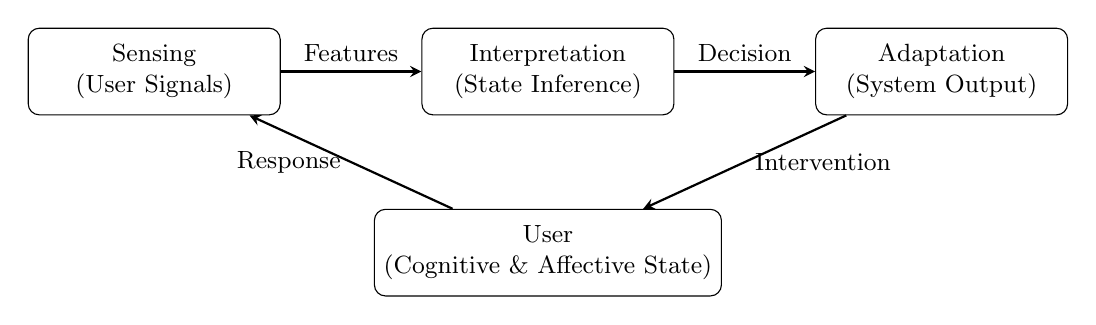
\begin{tikzpicture}[>=stealth, every node/.style={font=\small}]
        \node[draw, rounded corners, align=center, minimum width=3.2cm, minimum height=1.1cm] (sense) at (0,0) {Sensing\\(User Signals)};
        \node[draw, rounded corners, align=center, minimum width=3.2cm, minimum height=1.1cm] (infer) at (5,0) {Interpretation\\(State Inference)};
        \node[draw, rounded corners, align=center, minimum width=3.2cm, minimum height=1.1cm] (adapt) at (10,0) {Adaptation\\(System Output)};
        \node[draw, rounded corners, align=center, minimum width=3.8cm, minimum height=1.1cm] (user) at (5,-2.3) {User\\(Cognitive \& Affective State)};

        \draw[->, thick] (sense) -- node[above] {Features} (infer);
        \draw[->, thick] (infer) -- node[above] {Decision} (adapt);
        \draw[->, thick] (adapt) -- node[right] {Intervention} (user);
        \draw[->, thick] (user) -- node[left] {Response} (sense);
    \end{tikzpicture}
    \caption{General biocybernetic control loop used in physio-adaptive systems. The system senses user-related signals, infers a latent state, adapts the environment, and observes the user's response (adapted from \textcite{chiossi2023how}).}
    \label{fig:biocyberneticLoop}
\end{figure} 

The loop consists of three primary stages:
\begin{itemize}
    \item \textbf{Sensing (Input):} Continuous acquisition of user-related signals, such as physiological, behavioral, or contextual data.
    \item \textbf{Interpretation (Inference):} Transformation of these signals into features and inference of a latent user state or task-relevant condition.
    \item \textbf{Adaptation (Output):} Execution of a system response intended to support the user, stabilize performance, or reduce disruptive conditions.
\end{itemize}

In this thesis, the general loop is specified for flow support in competitive e-sports. During model development, sensing includes physiological signals such as ECG, EEG, and EDA, while the live evaluation focuses on ECG-derived HRV features and webcam-based affect features. In the interpretation stage, machine learning models map these features to \enquote{flow} or \enquote{non-flow} labels, following prior work on HRV-based flow classification \autocite{9296229}. In the adaptation stage, the system uses the inferred flow state to decide whether environmental interventions, such as shielding distracting notifications, should be triggered.

\subsubsection{Application in E-Sports: Shielding and the Measurement Paradox}
While office-based physio-adaptive designs often implement shielding mechanisms to suppress digital notifications \autocite{ubt_eref88160}, the application in competitive e-sports requires more domain-specific interventions. For instance, recent research in LoL has explored providing real-time data visualizations to support player training and performance monitoring \autocite{10.1145/3549506}. The necessity for such automated, non-intrusive interventions is driven by the inherent \enquote{obtrusiveness} of traditional measurement—whereby manual self-reporting would inevitably disrupt the very flow state the system is intended to protect. By integrating these measures directly into the gaming environment, the system maintains the player's immersion while providing actionable feedback or mitigating external distractions.

Because flow involves a recession of self-referential thought, mid-task surveys create a methodological paradox: the act of measuring the state requires the player to self-reflect, which inherently disrupts or terminates the flow experience \autocite{9296229, Moneta2012}. By utilizing the biocybernetic loop to provide \enquote{biologically transparent} monitoring, physio-adaptive systems can protect the user's immersion without the need for intrusive queries, mitigating the risk of distractions that can otherwise take a user up to 23 minutes to recover from \autocite{ubt_eref88160}.

\subsubsection{General Limitations of Physio-Adaptive Flow Support}
Although physio-adaptive systems offer a promising way to support flow without interruptive self-reports, their use also introduces methodological, technical, and contextual limitations. These limitations concern both existing NeuroIS approaches such as FlowShield and the specific transfer of such ideas to LoL.

\paragraph{Limitations of the FlowShield approach by Adam et al.}
The work by \textcite{ubt_eref88160} provides an important precedent for neuro-adaptive flow support and intelligent interruption management. However, its evaluation context differs substantially from competitive e-sports. The field evaluation demonstrates ecological relevance for knowledge-work settings, but it does not establish that the same intervention logic transfers directly to time-critical team games. In office work, notifications can often be delayed without immediate collective consequences; in LoL, however, communication may be strategically relevant within seconds. In addition, the FlowShield approach focuses on IT-mediated interruptions and flow support in work tasks, whereas e-sports involve rapid motor input, voice communication, emotional arousal, and volatile game states. Consequently, Adam et al.'s results should be treated as design guidance rather than direct evidence that autonomous shielding is suitable for competitive gaming. Their own discussion of limitations and future research also implies the need for further validation across contexts, longer-term use, and more diverse real-world settings \autocite{ubt_eref88160}.

\paragraph{Limitations in the LoL context.}
\begin{itemize}
    \item \textbf{Signal Ambiguity During Gameplay:} In LoL, physiological changes are not caused by cognitive flow alone. Team fights, rapid mouse and keyboard actions, voice-chat pressure, caffeine intake, and emotional reactions to deaths or objective losses can all alter ECG-derived HRV or facial affect. This creates a risk of false positives, where stress, physical activation, or frustration is misclassified as flow \autocite{fairclough2009fundamentals}.
    \item \textbf{Context Sensitivity of Interventions:} Autonomous adaptations can be problematic in LoL because the relevance of an interruption depends strongly on match context. A notification or Discord message may be irrelevant during farming but important during champion select, pauses, scrims, or team coordination. If the system suppresses information at the wrong moment, it may create \enquote{automation surprise} and reduce the player's perceived control \autocite{ubt_eref88160}.
    \item \textbf{Webcam and Environment Constraints:} Webcam-based affect recognition is sensitive to lighting, camera angle, occlusions from headsets or hands, and limited facial movement during intense concentration. In LoL, players may also look away from the camera toward secondary monitors or teammates, which can reduce the reliability of webcam-derived features.
    \item \textbf{Privacy and Competitive Integrity:} Continuous ECG and webcam monitoring may reveal sensitive information about stress, emotion, or performance pressure. In competitive LoL environments, such data require strict privacy protection and must be handled carefully so that monitoring does not conflict with player autonomy, team confidentiality, or tournament integrity \autocite{fairclough2009fundamentals}.
\end{itemize}
